% Options for packages loaded elsewhere
\PassOptionsToPackage{unicode}{hyperref}
\PassOptionsToPackage{hyphens}{url}
\PassOptionsToPackage{dvipsnames,svgnames,x11names}{xcolor}
%
\documentclass[
  letterpaper,
  DIV=11,
  numbers=noendperiod]{scrartcl}

\usepackage{amsmath,amssymb}
\usepackage{iftex}
\ifPDFTeX
  \usepackage[T1]{fontenc}
  \usepackage[utf8]{inputenc}
  \usepackage{textcomp} % provide euro and other symbols
\else % if luatex or xetex
  \usepackage{unicode-math}
  \defaultfontfeatures{Scale=MatchLowercase}
  \defaultfontfeatures[\rmfamily]{Ligatures=TeX,Scale=1}
\fi
\usepackage{lmodern}
\ifPDFTeX\else  
    % xetex/luatex font selection
    \setmainfont[]{Times New Roman}
    \setsansfont[]{Times New Roman}
\fi
% Use upquote if available, for straight quotes in verbatim environments
\IfFileExists{upquote.sty}{\usepackage{upquote}}{}
\IfFileExists{microtype.sty}{% use microtype if available
  \usepackage[]{microtype}
  \UseMicrotypeSet[protrusion]{basicmath} % disable protrusion for tt fonts
}{}
\makeatletter
\@ifundefined{KOMAClassName}{% if non-KOMA class
  \IfFileExists{parskip.sty}{%
    \usepackage{parskip}
  }{% else
    \setlength{\parindent}{0pt}
    \setlength{\parskip}{6pt plus 2pt minus 1pt}}
}{% if KOMA class
  \KOMAoptions{parskip=half}}
\makeatother
\usepackage{xcolor}
\setlength{\emergencystretch}{3em} % prevent overfull lines
\setcounter{secnumdepth}{-\maxdimen} % remove section numbering
% Make \paragraph and \subparagraph free-standing
\makeatletter
\ifx\paragraph\undefined\else
  \let\oldparagraph\paragraph
  \renewcommand{\paragraph}{
    \@ifstar
      \xxxParagraphStar
      \xxxParagraphNoStar
  }
  \newcommand{\xxxParagraphStar}[1]{\oldparagraph*{#1}\mbox{}}
  \newcommand{\xxxParagraphNoStar}[1]{\oldparagraph{#1}\mbox{}}
\fi
\ifx\subparagraph\undefined\else
  \let\oldsubparagraph\subparagraph
  \renewcommand{\subparagraph}{
    \@ifstar
      \xxxSubParagraphStar
      \xxxSubParagraphNoStar
  }
  \newcommand{\xxxSubParagraphStar}[1]{\oldsubparagraph*{#1}\mbox{}}
  \newcommand{\xxxSubParagraphNoStar}[1]{\oldsubparagraph{#1}\mbox{}}
\fi
\makeatother


\providecommand{\tightlist}{%
  \setlength{\itemsep}{0pt}\setlength{\parskip}{0pt}}\usepackage{longtable,booktabs,array}
\usepackage{calc} % for calculating minipage widths
% Correct order of tables after \paragraph or \subparagraph
\usepackage{etoolbox}
\makeatletter
\patchcmd\longtable{\par}{\if@noskipsec\mbox{}\fi\par}{}{}
\makeatother
% Allow footnotes in longtable head/foot
\IfFileExists{footnotehyper.sty}{\usepackage{footnotehyper}}{\usepackage{footnote}}
\makesavenoteenv{longtable}
\usepackage{graphicx}
\makeatletter
\def\maxwidth{\ifdim\Gin@nat@width>\linewidth\linewidth\else\Gin@nat@width\fi}
\def\maxheight{\ifdim\Gin@nat@height>\textheight\textheight\else\Gin@nat@height\fi}
\makeatother
% Scale images if necessary, so that they will not overflow the page
% margins by default, and it is still possible to overwrite the defaults
% using explicit options in \includegraphics[width, height, ...]{}
\setkeys{Gin}{width=\maxwidth,height=\maxheight,keepaspectratio}
% Set default figure placement to htbp
\makeatletter
\def\fps@figure{htbp}
\makeatother
% definitions for citeproc citations
\NewDocumentCommand\citeproctext{}{}
\NewDocumentCommand\citeproc{mm}{%
  \begingroup\def\citeproctext{#2}\cite{#1}\endgroup}
\makeatletter
 % allow citations to break across lines
 \let\@cite@ofmt\@firstofone
 % avoid brackets around text for \cite:
 \def\@biblabel#1{}
 \def\@cite#1#2{{#1\if@tempswa , #2\fi}}
\makeatother
\newlength{\cslhangindent}
\setlength{\cslhangindent}{1.5em}
\newlength{\csllabelwidth}
\setlength{\csllabelwidth}{3em}
\newenvironment{CSLReferences}[2] % #1 hanging-indent, #2 entry-spacing
 {\begin{list}{}{%
  \setlength{\itemindent}{0pt}
  \setlength{\leftmargin}{0pt}
  \setlength{\parsep}{0pt}
  % turn on hanging indent if param 1 is 1
  \ifodd #1
   \setlength{\leftmargin}{\cslhangindent}
   \setlength{\itemindent}{-1\cslhangindent}
  \fi
  % set entry spacing
  \setlength{\itemsep}{#2\baselineskip}}}
 {\end{list}}
\usepackage{calc}
\newcommand{\CSLBlock}[1]{\hfill\break\parbox[t]{\linewidth}{\strut\ignorespaces#1\strut}}
\newcommand{\CSLLeftMargin}[1]{\parbox[t]{\csllabelwidth}{\strut#1\strut}}
\newcommand{\CSLRightInline}[1]{\parbox[t]{\linewidth - \csllabelwidth}{\strut#1\strut}}
\newcommand{\CSLIndent}[1]{\hspace{\cslhangindent}#1}

\usepackage{booktabs}
\usepackage{longtable}
\usepackage{array}
\usepackage{multirow}
\usepackage{wrapfig}
\usepackage{float}
\usepackage{colortbl}
\usepackage{pdflscape}
\usepackage{tabu}
\usepackage{threeparttable}
\usepackage{threeparttablex}
\usepackage[normalem]{ulem}
\usepackage{makecell}
\usepackage{xcolor}
\KOMAoption{captions}{tableheading}
\makeatletter
\@ifpackageloaded{caption}{}{\usepackage{caption}}
\AtBeginDocument{%
\ifdefined\contentsname
  \renewcommand*\contentsname{Table of contents}
\else
  \newcommand\contentsname{Table of contents}
\fi
\ifdefined\listfigurename
  \renewcommand*\listfigurename{List of Figures}
\else
  \newcommand\listfigurename{List of Figures}
\fi
\ifdefined\listtablename
  \renewcommand*\listtablename{List of Tables}
\else
  \newcommand\listtablename{List of Tables}
\fi
\ifdefined\figurename
  \renewcommand*\figurename{Figure}
\else
  \newcommand\figurename{Figure}
\fi
\ifdefined\tablename
  \renewcommand*\tablename{Table}
\else
  \newcommand\tablename{Table}
\fi
}
\@ifpackageloaded{float}{}{\usepackage{float}}
\floatstyle{ruled}
\@ifundefined{c@chapter}{\newfloat{codelisting}{h}{lop}}{\newfloat{codelisting}{h}{lop}[chapter]}
\floatname{codelisting}{Listing}
\newcommand*\listoflistings{\listof{codelisting}{List of Listings}}
\makeatother
\makeatletter
\makeatother
\makeatletter
\@ifpackageloaded{caption}{}{\usepackage{caption}}
\@ifpackageloaded{subcaption}{}{\usepackage{subcaption}}
\makeatother

\ifLuaTeX
  \usepackage{selnolig}  % disable illegal ligatures
\fi
\usepackage{bookmark}

\IfFileExists{xurl.sty}{\usepackage{xurl}}{} % add URL line breaks if available
\urlstyle{same} % disable monospaced font for URLs
\hypersetup{
  pdftitle={EI Exit Analysis for Dissertation},
  pdfauthor={Maiko Hata},
  colorlinks=true,
  linkcolor={blue},
  filecolor={Maroon},
  citecolor={Blue},
  urlcolor={Blue},
  pdfcreator={LaTeX via pandoc}}


\title{EI Exit Analysis for Dissertation}
\author{Maiko Hata}
\date{}

\begin{document}
\maketitle


\section{Abstract}\label{abstract}

xxx

\section{Introduction}\label{introduction}

xxx

xxx

\section{\texorpdfstring{\textbf{Methods}}{Methods}}\label{methods}

\textbf{Independent variables (IV)}: xxx

\textbf{Dependent variables (DV)}: As you can see in Table 1, there are
ten exit categories under three general exit reason ``umbrellas''
(Hansen et al., 2016):

\begin{longtable}[l]{ll}
\caption{Table of Exit Reasons}\\
\toprule
Exit Reasons & Exit Category Codes\\
\midrule
Program completion & Category (C) 1: A child is no longer eligible for Part C prior to reaching age three \\
Exit at age three & C2: A child is exiting Part C and has been determined to be eligible for Part B \\
Exit at age three & C3: Part B eligible, continuing in Part C  \\
Exit at age three & C4: Not eligible for Part B, exit with referrals to other programs \\
Exit at age three & C5: Not eligible for Part B, exit with no referrals \\
\addlinespace
Exit at age three & C6: Part B eligibility not determined \\
Not receiving services  & C7: Deceased\\
Not receiving services  & C8: Moved out of state \\
Not receiving services  & C9: Withdrawal by parent (or guardian) \\
Not receiving services  & C10: Attempts to contact the parents and/or child were unsuccessful \\
\bottomrule
\end{longtable}

These ten reasons were collapsed into six reasons based on the scope of
this study and for logistical reasons. For example, ``Deceased'' is
beyond the scope of this study; one reason is not used in Oregon;
multiple codes were similar in nature to each other:

\begin{itemize}
\tightlist
\item
  Attempts to contact unsuccessful
\item
  Withdrawal by parent
\item
  Complete/not eligible for Part B
\item
  Moved out of state
\item
  Part B eligibility not determined
\item
  Part B eligible
\end{itemize}

\textbf{Preparatory work}: I prepared the data in a following manner:

\begin{enumerate}
\def\labelenumi{\arabic{enumi}.}
\tightlist
\item
  Created an Excel sheet from the national and Oregon data sets
\item
  Imported Excel sheet into RStudio
\item
  Collapsed/removed DVs
\item
  Collapsed data from multiple years into one aggregated data by race
\end{enumerate}

\textbf{Data Analysis}: I used chi-square goodness of fit test to
understand associations between children's race and their EI exit
reasons. Chi-square tests tell us if I can be confident that differences
in counts and expected counts are not due to chance. In other words,
chi-square tests can be used to evaluate if there is a statistically
significant relationship between two dichotomous or nominal variable.
However, they are not able to indicate the strength or the direction of
the relationship (Morgan et al., 2020).

First, I ran descriptive analysis of the national data set as an omnibus
test. For this, I used foundational statistical functions and chi-square
to test our null-hypothesis; there is no associations between children's
race and their exit reasons.

I then analyzed the association between the exit reason, ``Attempts to
Contact Unsuccessful'', using similar analysis. For this portion, we
looked at the association between two racial categories, Black/African
American and White infants/toddler groups, with ``Attempts to Contact
Unsuccessful''. We created 2x2 table for this analysis, complete with
the total number of exits. This was used to analyze the odd ratio and
Cohen's *h*. Odds ratio are commonly used for reporting the odds of one
outcome between two independent groups (Morgan, et al., 2020).

\section{Results}\label{results}

The initial exploration included exit data from 3,310,559 children who
exited the EI services between 2013 and 2022 nationally. Approximately
12.47\% of the children were Black/African American, while 50.64\% of
the children were reported as being White. This shows a possible
disproportionate representation of children, as census showed that
during these years, Black/African American and White children
represented approximately 14\% for Black/African American children under
the age of 18 and between 52\% to 49 \% for White children nationally
(The Annie E. Casey Foundation, 2024). When looking at children under
the age of six in 2022, the disparities widen: White children
represented only 46.5\% nationally, while Black/African American
children represented 12.7\% of the children under the age of 6
(Schneider \& Gibbs, 2023).

The chi-square omnibus test indicated that there was a statistically
significant association between children's race and their exit reasons,
X-squared (30, N = 3,310,559) = 52218.3, with a p-value of \textless{}
0.001

Looking specifically at the ``Attempts to Contact Unsuccessful''
category, approximately 13.5\% of Black/African American infants and
toddlers were disqualified from EI services nationally due to agencies
losing contact with families, while only about 5.98\% of White children
were disqualified for the same reason (Figure 1).

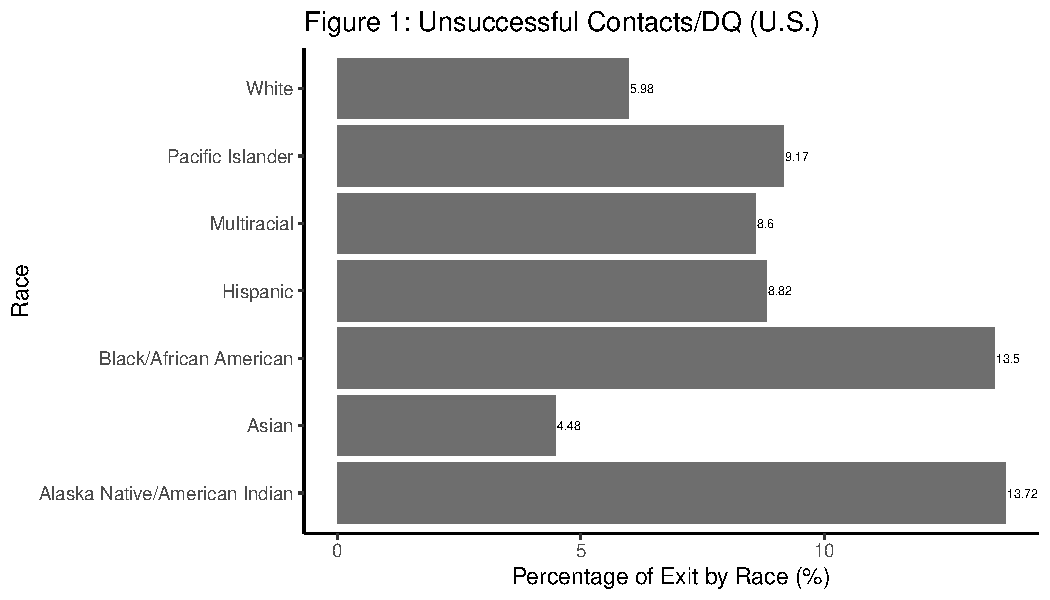
\includegraphics{v1_files/figure-pdf/unnamed-chunk-15-1.pdf}

When we look at the data at state level, the numbers change slightly.
Approximately 9.85\% of Black/African American infants and toddlers were
disqualified from EI services in Oregon due to agencies losing contact
with families, while only about 8.03\% of White children were
disqualified for the same reason in Oregon (Figure 2).

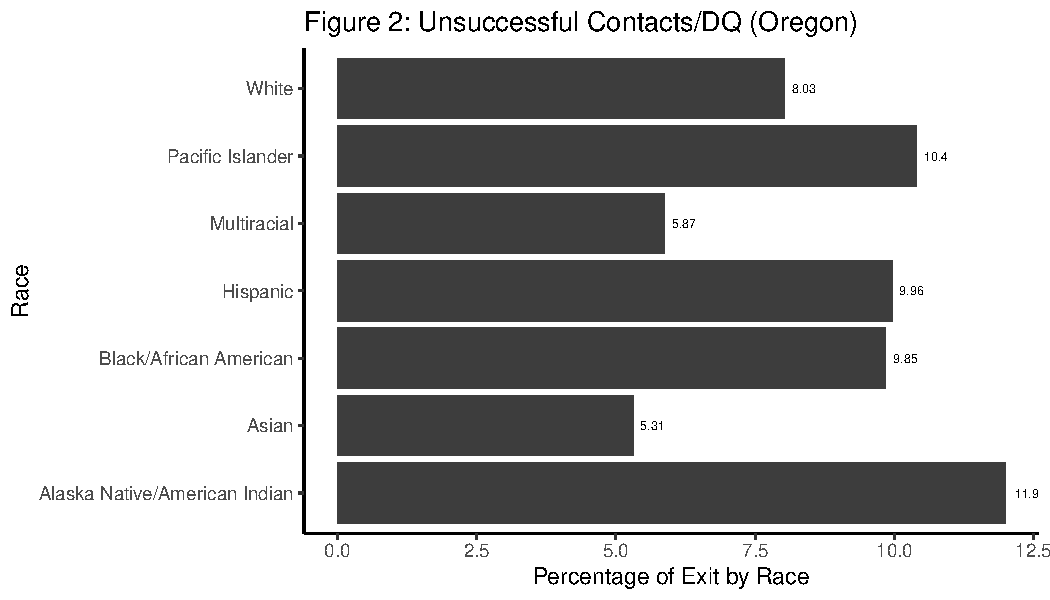
\includegraphics{v1_files/figure-pdf/unnamed-chunk-24-1.pdf}

The chi-square indicated that there was a statistically significant
association between children being Black/African American or White and
them leaving EI due to being disqualified nationally. The chi-square
test indicated, X-squared (222556.00, N = 2,088,058), \emph{p}
\textless{} 2.2e-16 or 0.0000000000000002 (\emph{p} \textless{} .001).

Because whether or not children were Black/African American or White and
whether they were likely to be disqualified from EI services due to
``Attempts to Contact Unsuccessful'' were both binary variables, we
computed an odds ratio as well.

In order to calculate the odds ratio to determine the relative
likelihood of the students being disqualified between the two groups, a
2x2 contingency table in a matrix format was created and analyzed. The
odds of Black infants and toddlers being disqualified from EI services
due to ``attempts to contact unsuccessful'' were significantly higher
than those for White infants and toddlers, with an odds ratio of
\textbf{2.46} (95\% CI {[}2.43, 2.48{]}). This indicates that Black
students were approximately 2.46 times more likely than White students
to be disqualified from EI services for this reason.

Cohen's \emph{h} was calculated to evaluate the effect size of the
analysis\textbf{.} The result indicated a small to medium effect size,
\emph{h} = 0.259. However, even though effect size shows the magnitude
of the difference, it is not necessarily considered to be a direct
indication of the importance of the findings (Morgan et al., 2020).

\section{Discussion}\label{discussion}

Our analysis revealed that the odds ratio for Black/African American
infants and toddlers to be disqualified from EI services due to
``Attempts to Contact Unsuccessful'' was 2.46 times higher when compared
to their White peers nationally. In addition, state-level data showed
smaller disparities between disqiualification rates between
Black/African American children and that of their White peers. However,
there are many limitations to this descriptive analysis.

First of all, we have to remember that race is not a predictive factor
for outcomes. At a quick glance, race seems to be associated with
inequity in EI service exit patterns. However, research following the
completion of the Human Genome Project has shown that race, from a
genetic standpoint, does not contribute to health inequities. Instead,
it is the environments experienced by racially minoritized communities
that play a significant role (Silverstein, 2015). Silverstein cited
Kittles (2015) in order to clarify this: ``the bulk of those disparities
are not due to any biological difference. The vast majority of health
disparities are due to social, behavioral, and environmental
components''. Race is merely one of the many descriptors for
individuals.~

In addition, as Crenshaw (1989) established in her seminal work, we must
take the framework of Intersectionality when conducting a research. This
type of oversimplified statistical analysis can contribute to reinforce
the status-quo where race is quickly to be blamed, rather than the
complex environments and multiple layers of identities that members of
marginalized communities live in.

The smaller disparity between racial groups in Oregon in terms of
disqualification rate could be due to the state's limited diversity,
meaning we simply don't have enough data. This makes it challenging to
conduct quantitative studies on marginalized populations, even though
research is so urgently needed for that very reason.

Last but not least, researchers have argued that quantitative methods
are inequitable, as ``the history of quant methods is inseparable from
eugenics movement'' (p.~4, Castillo \& Strunk, 2024) and that it stems
from and reinforces inequity. QuantCrit philosophy are based and expands
on the centrality of racism and the lack of neutrality in numbers and
categories. Going forward, it would be extremely important to remember
these tenets and to approach data collection, categorization and
analysis with equity and justice as the central philosophy.

\newpage

\section{References}\label{references}

Annie E. Casey Foundation. (2024, July). Child population by race and
ethnicity. KIDS COUNT Data Center.
\url{https://datacenter.aecf.org/data/tables/103-child-population-by-race-and-ethnicity\#detailed/1/any/false/1095,2048,574,1729,37,871,870,573,869,36/72,66,67,8367,69,70,71,12/423,424}

Castillo, W. \& Strunk, K. (2024, November 15). How to QuantCrit
{[}PowerPoint slides{]}.
\url{https://www.sree.org/critical-perspectives}

Crenshaw, K. (1989). Demarginalizing the intersection of race and sex: A
Black feminist critique of antidiscrimination doctrine, feminist theory
and antiracist politics. University of Chicago Legal Forum, 1989(1),
139-167.

Early Childhood Technical Assistance Center {[}ecta{]}, (2023, October
6). \emph{Part C of IDEA}. ecta.
\url{https://ectacenter.org/partc/partc.asp}

Individuals with Disabilities Education Act, 20 U.S.C. § 1400 (2004).

Morgan, G.A., Barrett, K.C., Leech, N.L., \& Gloeckner, G.W. (2020).
\emph{IBM SPSS for introductory statistics: Use and interpretation.}
Routledge.

Morgan, P. L., Farkas, G., Hillemeier, M. M., \& Maczuga, S. (2012). Are
minority children disproportionately represented in Early Intervention
and Early Childhood Special Education? Educational Researcher, 41(9),
339--351. https://doi.org/10.3102/0013189X12459678

OpenAI. (2024). \emph{ChatGPT} {[}Large language model{]}. Provided code
assistance. Retrieved from \url{https://chat.openai.com/}

Romano, S.D. (2006). Historical perspectives. In G. M. Foley \& J.D.
Hochman (Eds.), \emph{Mental health in early intervention: Achieving
unity in principles and practice} (pp.~33-58). Baltimore: Paul H.
Brookes Publishing Company.

Schneider, A. \& Gibbs, H. (2023, December 14). Data dashboard: An
overview of child care and early learning in the United States. The
Center for American Progress.
\url{https://www.americanprogress.org/article/data-dashboard-an-overview-of-child-care-and-early-learning-in-the-united-states/}

Silverstein, J. (2015, April 15). Genes don't cause racial-health
disparities, society does. The Atlantic.
\url{https://www.theatlantic.com/health/archive/2015/04/genes-dont-cause-racial-health-disparities-society-does/389637/}~

\newpage

We used R version 4.4.1 (R Core Team, 2024) and the following R
packages: DT v. 0.33 (Xie et al., 2024), epitools v. 0.5.10.1 (Aragon,
2020), gt v. 0.11.1 (Iannone et al., 2024), gtsummary v. 2.0.3 (Sjoberg
et al., 2021), here v. 1.0.1 (Müller, 2020), janitor v. 2.2.0 (Firke,
2023), kableExtra v. 1.4.0 (Zhu, 2024), knitr v. 1.48 (Xie, 2014, 2015,
2024a), lme4 v. 1.1.35.5 (Bates et al., 2015), pwr v. 1.3.0 (Champely,
2020), rcompanion v. 2.4.36 (Mangiafico, 2024), reactable v. 0.4.4 (Lin,
2023), rio v. 1.2.3 (Chan et al., 2023), rmarkdown v. 2.28 (Allaire et
al., 2024; Xie et al., 2018, 2020), sjPlot v. 2.8.16 (Lüdecke, 2024),
tidylog v. 1.1.0 (Elbers, 2024), tidyverse v. 2.0.0 (Wickham et al.,
2019), tinytex v. 0.53 (Xie, 2019, 2024b).

\phantomsection\label{refs}
\begin{CSLReferences}{1}{0}
\bibitem[\citeproctext]{ref-rmarkdown2024}
Allaire, J., Xie, Y., Dervieux, C., McPherson, J., Luraschi, J., Ushey,
K., Atkins, A., Wickham, H., Cheng, J., Chang, W., \& Iannone, R.
(2024). \emph{{rmarkdown}: Dynamic documents for r}.
\url{https://github.com/rstudio/rmarkdown}

\bibitem[\citeproctext]{ref-epitools}
Aragon, T. J. (2020). \emph{{epitools}: Epidemiology tools}.
\url{https://CRAN.R-project.org/package=epitools}

\bibitem[\citeproctext]{ref-lme4}
Bates, D., Mächler, M., Bolker, B., \& Walker, S. (2015). Fitting linear
mixed-effects models using {lme4}. \emph{Journal of Statistical
Software}, \emph{67}(1), 1--48.
\url{https://doi.org/10.18637/jss.v067.i01}

\bibitem[\citeproctext]{ref-pwr}
Champely, S. (2020). \emph{{pwr}: Basic functions for power analysis}.
\url{https://CRAN.R-project.org/package=pwr}

\bibitem[\citeproctext]{ref-rio}
Chan, C., Leeper, T. J., Becker, J., \& Schoch, D. (2023). \emph{{rio}:
A swiss-army knife for data file i/o}.
\url{https://cran.r-project.org/package=rio}

\bibitem[\citeproctext]{ref-tidylog}
Elbers, B. (2024). \emph{{tidylog}: Logging for {``{dplyr}''} and
{``{tidyr}''} functions}.
\url{https://CRAN.R-project.org/package=tidylog}

\bibitem[\citeproctext]{ref-janitor}
Firke, S. (2023). \emph{{janitor}: Simple tools for examining and
cleaning dirty data}. \url{https://CRAN.R-project.org/package=janitor}

\bibitem[\citeproctext]{ref-gt}
Iannone, R., Cheng, J., Schloerke, B., Hughes, E., Lauer, A., Seo, J.,
Brevoort, K., \& Roy, O. (2024). \emph{{gt}: Easily create
presentation-ready display tables}.
\url{https://CRAN.R-project.org/package=gt}

\bibitem[\citeproctext]{ref-reactable}
Lin, G. (2023). \emph{{reactable}: Interactive data tables for r}.
\url{https://CRAN.R-project.org/package=reactable}

\bibitem[\citeproctext]{ref-sjPlot}
Lüdecke, D. (2024). \emph{{sjPlot}: Data visualization for statistics in
social science}. \url{https://CRAN.R-project.org/package=sjPlot}

\bibitem[\citeproctext]{ref-rcompanion}
Mangiafico, S. S. (2024). \emph{{rcompanion}: Functions to support
extension education program evaluation}. Rutgers Cooperative Extension.
\url{https://CRAN.R-project.org/package=rcompanion/}

\bibitem[\citeproctext]{ref-here}
Müller, K. (2020). \emph{{here}: A simpler way to find your files}.
\url{https://CRAN.R-project.org/package=here}

\bibitem[\citeproctext]{ref-base}
R Core Team. (2024). \emph{{R}: A language and environment for
statistical computing}. R Foundation for Statistical Computing.
\url{https://www.R-project.org/}

\bibitem[\citeproctext]{ref-gtsummary}
Sjoberg, D. D., Whiting, K., Curry, M., Lavery, J. A., \& Larmarange, J.
(2021). Reproducible summary tables with the gtsummary package.
\emph{{The R Journal}}, \emph{13}, 570--580.
\url{https://doi.org/10.32614/RJ-2021-053}

\bibitem[\citeproctext]{ref-tidyverse}
Wickham, H., Averick, M., Bryan, J., Chang, W., McGowan, L. D.,
François, R., Grolemund, G., Hayes, A., Henry, L., Hester, J., Kuhn, M.,
Pedersen, T. L., Miller, E., Bache, S. M., Müller, K., Ooms, J.,
Robinson, D., Seidel, D. P., Spinu, V., \ldots{} Yutani, H. (2019).
Welcome to the {tidyverse}. \emph{Journal of Open Source Software},
\emph{4}(43), 1686. \url{https://doi.org/10.21105/joss.01686}

\bibitem[\citeproctext]{ref-knitr2014}
Xie, Y. (2014). {knitr}: A comprehensive tool for reproducible research
in {R}. In V. Stodden, F. Leisch, \& R. D. Peng (Eds.),
\emph{Implementing reproducible computational research}. Chapman;
Hall/CRC.

\bibitem[\citeproctext]{ref-knitr2015}
Xie, Y. (2015). \emph{Dynamic documents with {R} and knitr} (2nd ed.).
Chapman; Hall/CRC. \url{https://yihui.org/knitr/}

\bibitem[\citeproctext]{ref-tinytex2019}
Xie, Y. (2019). {TinyTeX}: A lightweight, cross-platform, and
easy-to-maintain LaTeX distribution based on TeX live. \emph{TUGboat},
\emph{40}(1), 30--32.
\url{https://tug.org/TUGboat/Contents/contents40-1.html}

\bibitem[\citeproctext]{ref-knitr2024}
Xie, Y. (2024a). \emph{{knitr}: A general-purpose package for dynamic
report generation in r}. \url{https://yihui.org/knitr/}

\bibitem[\citeproctext]{ref-tinytex2024}
Xie, Y. (2024b). \emph{{tinytex}: Helper functions to install and
maintain TeX live, and compile LaTeX documents}.
\url{https://github.com/rstudio/tinytex}

\bibitem[\citeproctext]{ref-rmarkdown2018}
Xie, Y., Allaire, J. J., \& Grolemund, G. (2018). \emph{R markdown: The
definitive guide}. Chapman; Hall/CRC.
\url{https://bookdown.org/yihui/rmarkdown}

\bibitem[\citeproctext]{ref-DT}
Xie, Y., Cheng, J., \& Tan, X. (2024). \emph{{DT}: A wrapper of the
JavaScript library {``{DataTables}''}}.
\url{https://CRAN.R-project.org/package=DT}

\bibitem[\citeproctext]{ref-rmarkdown2020}
Xie, Y., Dervieux, C., \& Riederer, E. (2020). \emph{R markdown
cookbook}. Chapman; Hall/CRC.
\url{https://bookdown.org/yihui/rmarkdown-cookbook}

\bibitem[\citeproctext]{ref-kableExtra}
Zhu, H. (2024). \emph{{kableExtra}: Construct complex table with
{``{kable}''} and pipe syntax}.
\url{https://CRAN.R-project.org/package=kableExtra}

\end{CSLReferences}




\end{document}
